%%%%%%%%%%%%%%%%%%
%  placeholders  %
%%%%%%%%%%%%%%%%%%

\newcommand{\uni}{Technical University of Munich}
\newcommand{\department}{TUM Department of Informatics}
\newcommand{\chair}{Chair for Applied Software Engineering}
\newcommand{\city}{Munich}
\newcommand{\country}{Germany}

% TODO: Replace with your information
\title{Predicting competition performance of age group swimmers}
\newcommand{\authorname}{Miriam Ansch\"utz}
\newcommand{\email}{m.anschuetz@tum.de}

\documentclass[conference]{IEEEtran}
\IEEEoverridecommandlockouts
% The preceding line is only needed to identify funding in the first footnote. If that is unneeded, please comment it out.
\usepackage[numbers]{natbib}
\usepackage{amsmath,amssymb,amsfonts}
\usepackage{algorithmic}
\usepackage{graphicx}
\usepackage{tabularx}
\usepackage{multirow}
\usepackage{booktabs}
\usepackage{caption}
\usepackage{etoolbox}
\makeatletter
\patchcmd{\@makecaption}
  {\scshape}
  {}
  {}
  {}
\makeatother
\def\tablename{Table}
\usepackage{placeins}
\usepackage{makecell}
\usepackage{textcomp}
\usepackage{xcolor}
\usepackage{url}
\def\BibTeX{{\rm B\kern-.05em{\sc i\kern-.025em b}\kern-.08em
    T\kern-.1667em\lower.7ex\hbox{E}\kern-.125emX}}
    
\begin{document}

\author{
	\IEEEauthorblockN{\authorname}
	\IEEEauthorblockA{\textit{\department, \chair} \\
	\textit{\uni}\\
	\city, \country \\
	\email}}

\maketitle

\begin{abstract}
%\begin{itemize}
%	\item Make the readers interested and provide all the necessary information for the readers to decide if the content is relevant to them.
%	\item Summarize the major aspects of your report in a few sentences.
%	\item Describe the problem you are approaching and what solution you have developed.
%	\item Describe the relevance of your work and why your report is a valuable addition to the seminar.
%	\item Do not include lengthy descriptions, abbreviations, figures, unnecessary adverbs, citations or references to other literature.
%	\item Do Not Use Symbols, Special Characters, Footnotes, or Math in Paper Title or Abstract.
%\end{itemize}
Age group swimmers' performance is hard to predict as their performance is highly dependent on their current training status and body development. In this paper, we propose an Android application that helps coaches to estimate the performance of their athletes. Therefore, the coaches can measure the 50m freestyle times in training and use our app to predict the corresponding 100m and 200m freestyle time. We use a linear regression network that predicts these times based on the 50m time as well as the swimmer's age and training age, i.e. how long the swimmer has been training on a competitional level. With this approach, we can predict the 100m time with an error of 1.83s and the 200m time with an error of 7.97 on average. We encounter problems due to non-professional swimmers being unreliable with regards to their competition performance. Moreover, our dataset provides insufficient information about the swimmer and his training status. Nevertheless, we consider our approach as a valuable contribution to help coaches of non-professional junior swimmers to estimate their swimmers' performances.
\end{abstract}

%%%%%%%%%%%%%%%%%%%%%%%%%
%  General Information  %
%%%%%%%%%%%%%%%%%%%%%%%%%

% Keep the slides from the Kick-Off Meeting in mind.
% The goal of the seminar is to take a look at applications of machine learning in real world scenarios or with real world applications.
% We want to take theoretical concepts and new approaches and apply them to existing or emerging problems.
% It is important that you document your process, collect citations, the process how you got to the results is as valuable as the end result.
% The seminar be about 6 pages (+ bibliography) long. It should summarize your literature research and related work.
% - Related practical work e.g. frameworks, tools, applications
% - Related academic literature such as papers and books
% - Showcases your proposed solution and prototype
% - Describe the implementation, challenges, and interesting technical details
% - Showcase why your prototype is a relevant for consumers or research
% - Details possible future work

\section{Introduction}

%\begin{itemize}
%	\item Establish the scope of your report
%	\item Define the most important background information and the current state of the field your research is placed in
%	\item Describe your research approach, the problem you are trying to solve
%	\item Highlight potential outcomes that can be established as part of the report
%	\item Outline the structure of your paper
%\end{itemize}

% organisation into heats -> registration time important
In swimming competitions, every swimmer has his lane; thus, the competition is organised in heats. These heats are ordered by speed so the first heats are the slowest and the last are the fastest. To organise these heats, the coaches have to submit estimated times when registering their swimmer for the respective competition. A swimmer has a psychological benefit if he swims in a heat together with swimmers of the same speed; thus, it is essential that the estimated time is correct. For junior swimmers, however, it is hard to estimate the correct time as junior swimmers react strongly to stress and environmental influences whats makes them more unreliable in competitions. Moreover, a new training input, e.g. an intense training camp, or growing up has a stronger impact for junior swimmers than for professionals thus, their performance changes more often. A possible solution for this could be to measure the times in training. For short distances this works very well, for longer distances, however, the training and competition times diverge. In this paper, we propose a mobile application that helps swim trainers to find the best registration times. The coaches can measure the 50m freestyle time in training and use the app to get the corresponding 100 and 200m freestyle times. To do so, we use a machine learning model that predicts the 100 and 200m time based on the 50m time as well as the age, gender and training age of the athlete. Besides, we investigate the relationship of different swimming distances and their times with a focus on junior swimmers.\\
This paper is structured as follows: In section \ref{sec:rel_work} we will explain the sports theory background and compare our work to current research. In section \ref{sec:contribution} we explain our approach, i.e. the dataset used for training, the machine learning model and the mobile application in detail and we evaluate the machine learning performance and the resulting app in section \ref{sec:results}.

\section{Related Work and background} \label{sec:rel_work}
In the following, we will explain relevant sport theory concepts that our work is based upon and compare our approach to related research.
%\begin{itemize}
%	\item Put your work in the context of the related research in the field.
%	\item Summarize related literature and the relationship between the related work.
%	\item Identify missing parts in current research or missing opportunities in applying related work.
%	\item Reference possible future work of other papers to support your work, e.g.: \cite{bruegge2009object}.
%	\item Judge existing reproach by its reproducibility and credibility.
%	\item Do not just cite for the number of citations, each citation should have its justification your can defend if needed.
%\end{itemize}
\subsection{Sports theory background}
There are three different ways of energy provision in the muscles. The first and most efficient energy production comes from ATP that is stored in the cells. However, this only works for about 2 seconds. When this storage is depleted, the body generates ATP from glycogen that is also stored in the muscle cells. This way of energy provision is also very efficient but does not last for long, either. The long-time energy is produced by consuming oxygen (aerobic energy production) \cite{Bompa.2018}. Figure \ref{fig:energy_provision} shows how the energy in
the muscle cells is provided over time.  In the first seconds, the energy comes from the ATP stored in the muscle cells, and the anaerobic energy production starts.  The longer the activity lasts, the more energy comes from aerobic production. 50m sprints last for about 25s to 50s thus more than 60\% of the energy comes from anaerobic energy production \cite{Dr.PatriziaMayerHaralOchwatweitereBSVDozenten.2007} . As this energy production is independent of oxygen and its transport, the energy provision is independent of fatigue; thus, the 50m times in training are close to those in competition.
\begin{figure}[ht]
    \centering
    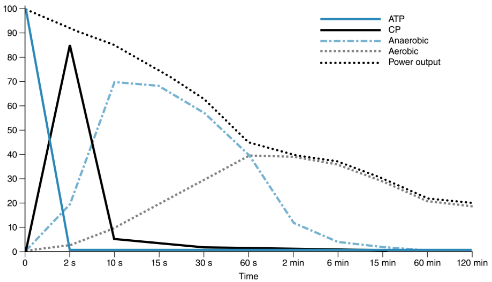
\includegraphics[scale=0.5]{visualisation/energy_provision.png}
    \caption{Energy provision by time \cite{Bompa.2018}}
    \label{fig:energy_provision}
\end{figure}
In general, a single training session can be split into multiple phases. During and shortly after the training session, the athlete is fatigued. After the training session has ended, the recovery starts. Recovery includes restoring energy stores in the muscles and reduce the lactic acid in the blood circulation. After many training sessions, the athlete's body starts to adapt to the constant exertion, i.e. the energy stores in the muscles increase or the heart muscle becomes stronger. This adaption process leads to improvement of the athlete's performance \cite{Bompa.2018.adaption}. Figure \ref{fig:training_improvement} visualises this adaption effect. The blue curve shows the performance of the athlete. With every stimulus, i.e. training session, the performance reduces to a minimum due to fatigue. After recovery, the maximum performance increases due to adaption.
\begin{figure}[ht]
    \centering
    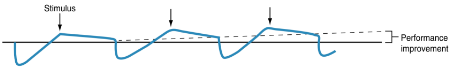
\includegraphics[scale=0.5]{visualisation/training_improvement.png}
    \caption{Performance improvement by continuous training \cite{Bompa.2018.compensation}}
    \label{fig:training_improvement}
\end{figure}
\subsection{Critical power concept} \label{critical_power}
In sports theory, critical power is the maximum rate that can be sustained for a very long time without fatigue \cite{Monod.1965,Hill.1993}. \citet{Monod.1965} introduced this concept and showed in their study that muscle power output and time to exhaustion follows a hyperbolic relationship while the total work performed is linearly connected to the time to exhaustion. Therefore, the critical power can be used as an indicator of the athlete's endurance and anaerobic capacity. With this indicator, coaches can optimise their training by setting loads and intensity in the aerobic area and evaluating the athlete's anaerobic performance without employing expensive material \cite{Dekerle.2002}. Other studies have shown that these concepts are applicable for swimming in general \cite{Wakayoshi.1992} and also for junior swimmers \cite{Hill.1995}. The critical power concept is of interest for our work as it gives us an idea of how the distances and the corresponding times are related.
\subsection{Machine learning for swim result prediction}
To the best of our knowledge, there is no related work that uses the same approach as we propose. However, some papers use similar data representation or try to achieve the same result but based on a different setting.\\
\citet{Silva.2007} use neural nets to predict the swimmer’s performance in 200m individual medley and 400m freestyle based on how the swimmer performs in multiple fitness, strength and flexibility tests. The authors submitted 138 junior swimmers of national level to four test categories: kinanthropometric, general functional and specific functional tests as well as an evaluation of their swimming technique. With the results of these tests, they predict the swimmer’s competition performance using Artificial neural nets. Moreover, they determine the physical factors that affect this performance the most. Although the ground truth, i.e. the data the model uses for training, is different from our, the machine learning approach itself is similar to our approach: They train a multilayer perceptron with one hidden layer and mean-squared error as loss function. \citet{EdelmannNusser.2002} use this machine learning approach as well. However, they try to predict the Olympic 200m backstroke performance of only a single swimmer. Therefore, their training data contains specific knowledge about the amount and intensity of training in the weeks before the respective competition. With this approach, they were able to predict the performance with a mean-absolute error of $\pm 0.62s$.\\
In order to predict how junior swimmers perform when they are older,, \citet{Xie.2015} divide 12- and 13-year-old top swimmers from the US into four performance level: the top 25\%, 25\%-50\%, 50\%-75\% and the last 25\%. A swimmer is represented by a single record of \texttt{(stroke, course, age, time, powerpoint)} where the powerpoint is a score that relates the swimmer's performance to other performances in this age group. Using SVM and neural networks, they determine the level change rate that is the probability that the swimmer will (still) be in the top-level when he is 18 years old. 
%%\begin{itemize}
%	\item Lead up to your contributions.
%	\item Describe your research process.
%	\item Start with theoretical work and work yourself to its applications in your reproach report.
%	\item Document your implementation and solution to the problem described in previous sections.
%	\item Discuss your data collection, training or implementation approach and highlight interesting technical details.
%	\item Feel free to add more sections or subsections and rename existing sections e.g. the Contributions section as you need.
%\end{itemize}
\section{Design and implementation}\label{sec:contribution}
 




%\section{Results \& Discussion}\label{sec:results}

%\begin{itemize}
%	\item Describe your results in a clrear and understandable way.
%	\item Clearly differentiate between what you have achieved and what you have build upon.
%	\item Ideally add some sort of visual representation of your result that underlines the progress you have made during the research project.
%	\item Make sure that the results are reproducible by your reader if needed
%	\item Critically discuss your results.
%	\item Did you achieve what you set out to do?
%	\item What are the strengths and weaknesses of your research?
%\end{itemize}
In this section, we discuss our dataset, evaluate our machine learning model and present our final mobile application.
\subsection{Dataset}


\subsection{Android application}

\section{Data generation}\label{sec:data_gen}
As we could not find a dataset that matches our requirements, we generate a new dataset using competition result published by the DSV (Deutscher Schwimm-Verband e.V.). All swimmers that are eight years or older and take part in competitions in Germany must register at the DSV. The DSV publishes all official competition results as well as information about registered swimmers online \footnote{\url{http://www.dsv.de/schwimmen/wettkampf-national/schwimmerabfrage/}, accessed 02.01.2020}; thus, we can access a considerable amount of data for our dataset.\\
Similar to the records in \textit{Prediction on Performance of Age Group Swimming Using Machine Learning} by \citet{Xie.2015} our dataset contains records that look like this: \texttt{(gender, age, training age, 50m time, 100m time, 200m time)}. To get a continuous representation of our data, we express all times in seconds with two decimal places.\\
We include the gender and the age of the swimmer as boys and girls develop differently at different ages. \citet{Golle.2015} showed in their study that the fitness performance improves when children get older. While boys outperformed girls of the same age-group in upper-extremity muscular power and endurance, girls performed better in flexibility test. All of the three aforementioned physical aspects are important for swimmers; thus, we expect different performances by swimmers of different age groups and gender. We use the swimmer's age group to determine his age instead of his actual age at the respective competition. Our dataset covers ages from nine to 14 years\\
The training age describes how long the swimmer has been training competitive swimming. The longer the swimmer has been training, the better is the swimmer's endurance and his technique as explained in section \ref{sec:sport_theory}. On top of that, he gained experience in competitions; thus, he may be less nervous during competition. In our dataset, we consider training ages ranging from one to seven years.\\
\citet{Wakayoshi.1992} have shown that for college swimmers, the distance and the corresponding time have a linear connection thus we can calculate the longer distance time based on any shorter distance. However, \citet{Golle.2015} observed a curvilinear improvement in upper-body strength and endurance for older junior swimmers. Putting this together, we expect the correlation between 50m, 100m, and 200m time to be non-linear, dependent on the age, training age and gender of the swimmer.\\
Using the aforementioned considerations, we generate two different datasets, a training and a test dataset. The training dataset consists of 116 samples with 49 female and 67 male swimmers. The test dataset contains 19 samples, ten of which are female. The swimming times in the dataset were achieved at the same competition on the same weekend in a 25m pool.
\begin{figure}[ht]
    \centering
    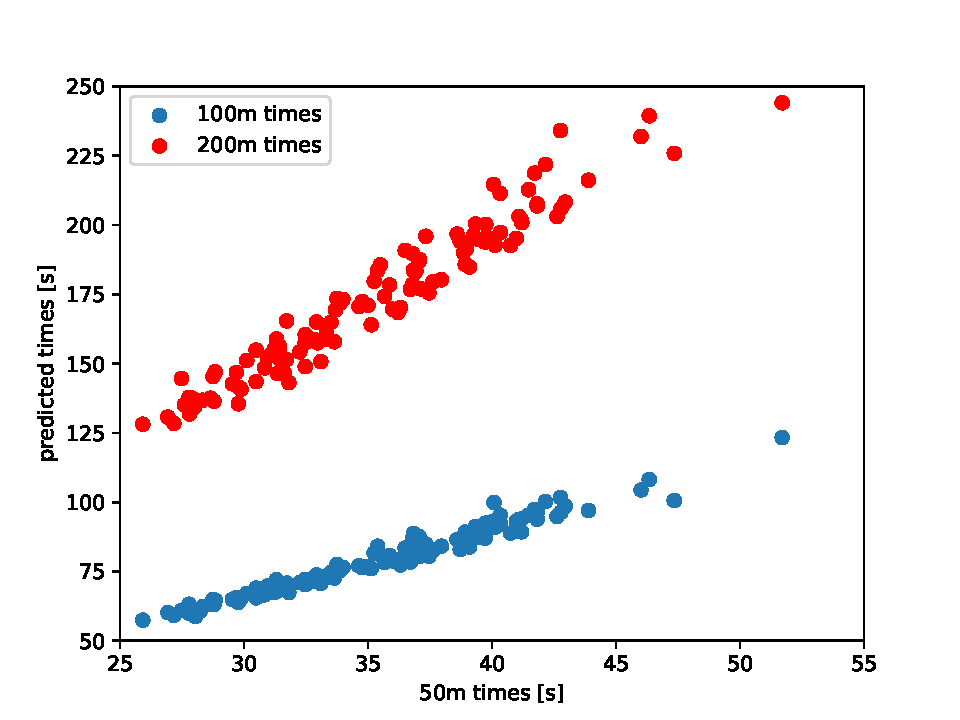
\includegraphics[scale=0.5]{visualisation/training_data.pdf}
    \caption{Training data: correlation of 50m and longer distance times}
    \label{fig:training_data}
\end{figure}
Figures \ref{fig:training_data} and \ref{fig:test_data} show the correlation of 50m and the longer distance times. In order to plot the samples in 2D, we omit the information about the swimmer. We can see that the times have a strong linear correlation with a Pearson correlation coefficient of $0.983$ for the 100m training data and $0.972$ for the 200m training data. Therefore, our initial assumption that age is essential for the prediction was wrong. Even for junior swimmers, the times follow a linear correlation as introduced by the critical power concept in section \ref{critical_power}, independent of the age, the training age or the gender.\\
\begin{figure}[ht]
    \centering
    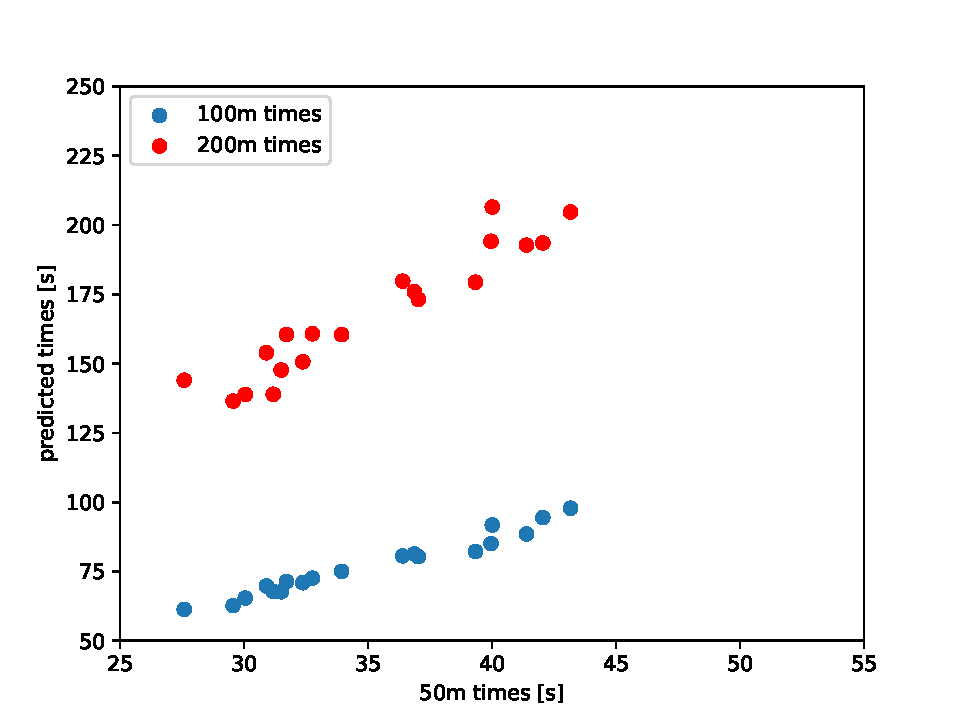
\includegraphics[scale=0.5]{visualisation/test_data.pdf}
    \caption{Test data: correlation of 50m and longer distance times}
    \label{fig:test_data}
\end{figure}
Also, we observe a higher variance in the long-distance times for higher 50m times. As we can see in Figure \ref{fig:training_age}, these higher 50m times are mostly from swimmers that are in their first or second training year. These swimmers have less competition experience or a rather bad technique. Moreover, young swimmers are often very nervous at competitions; thus, they make mistakes more likely. This makes it harder to predict their performance. The better a swimmer is, i.e. the longer he trains and the better his technique is, the more reliable his performance will be.
\begin{figure}[ht]
    \centering
    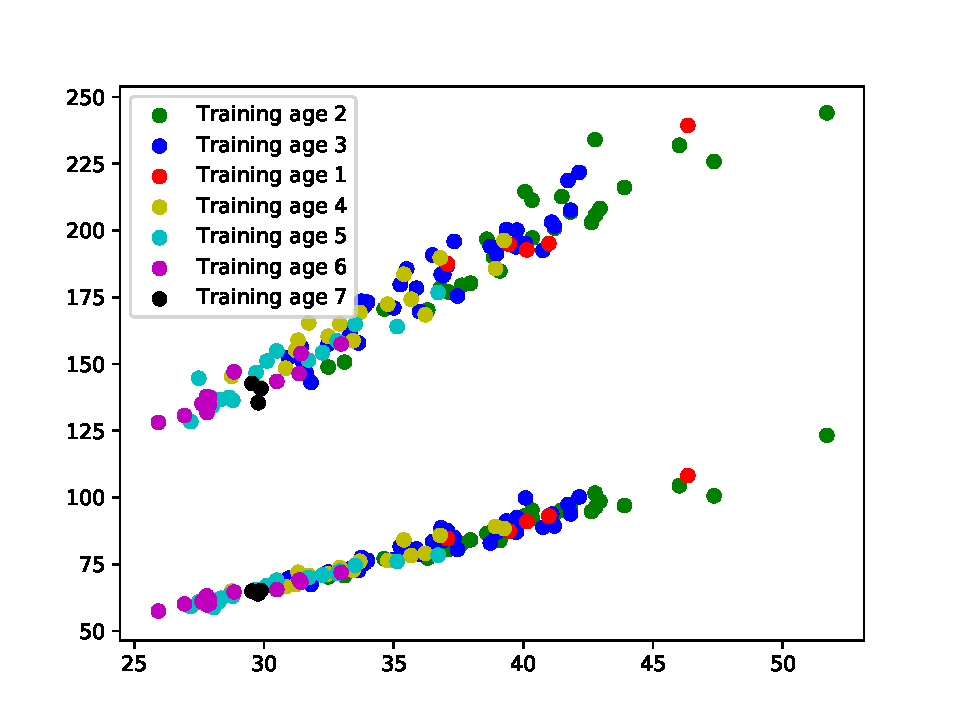
\includegraphics[scale=0.5]{visualisation/training_data_train_ages.pdf}
    \caption{Training data: influence of training age}
    \label{fig:training_age}
\end{figure}
\section{Machine learning approach}\label{sec:machine_learning}
\begin{figure*}[ht]
\begin{minipage}{0.62\textwidth}
\begin{tabular}{|c|c|c|c|}\hline
    Model &Training data&Test data&Error  \\\hline
    \makecell{
\includegraphics[scale=0.5]{visualisation/blue_square.png}\\original}&swimmer info, 50m&swimmer info, 50m&7.97\\\hline
    
\includegraphics[scale=0.5]{visualisation/yellow_circle.png}&\makecell{swimmer info, 50m,\\ true 100m}& \makecell{swimmer info, 50m,\\ true 100m}&5.77\\\hline
    
\includegraphics[scale=0.5]{visualisation/red_circle.png}&\makecell{swimmer info, 50m,\\ true 100m}&\makecell{swimmer info, 50m,\\ predicted 100m}&8.30\\\hline
    
\includegraphics[scale=0.5]{visualisation/green_triangle.png}&\makecell{swimmer info, 50m,\\ predicted 100m}&\makecell{swimmer info, 50m,\\ predicted 100m}&7.67\\\hline
\end{tabular}
\end{minipage}
\begin{minipage}{0.38\textwidth}
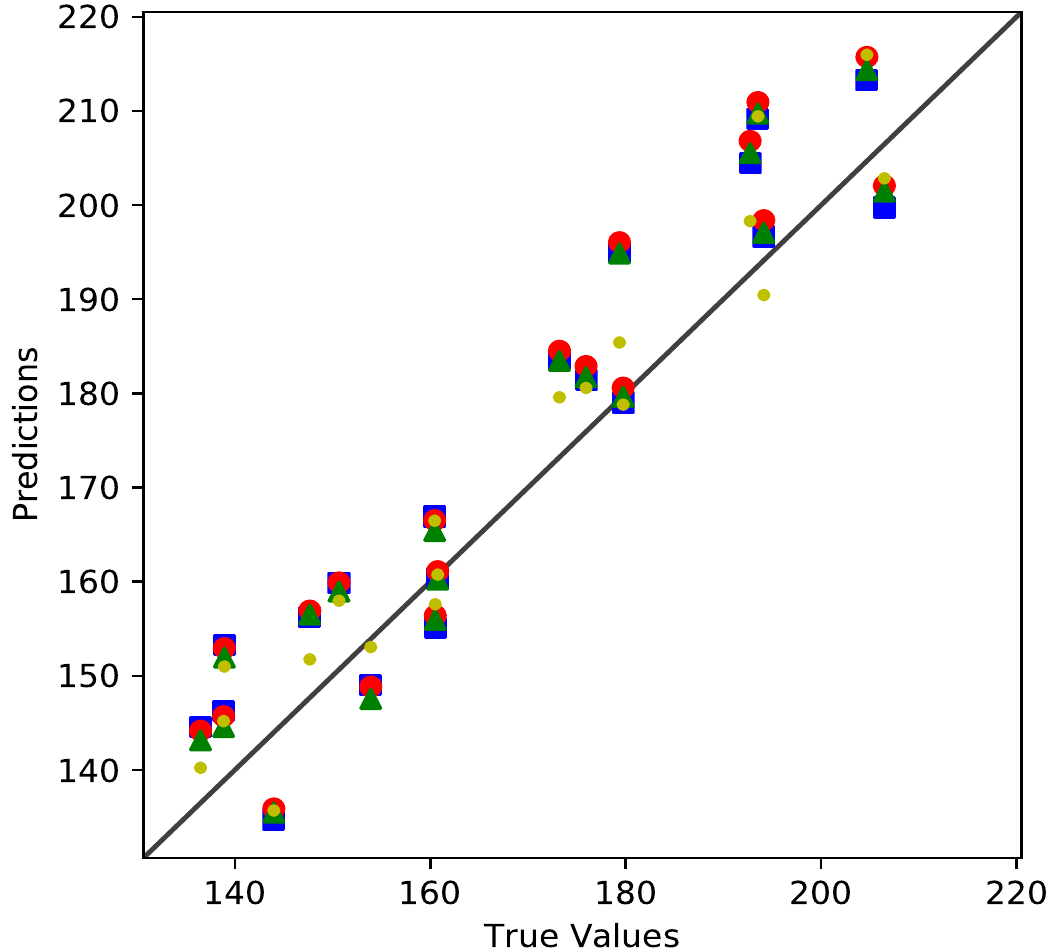
\includegraphics[width=\textwidth]{visualisation/eval_200m_variations.png}
\end{minipage}
\caption{Comparison of different 200m approaches}
\label{fig:200m_variations}
\end{figure*}
Using these datasets, we train machine learning models to predict the longer distance times. We use Tensorflow\footnote{\url{https://www.tensorflow.org/} accessed 03.01.2020} for training our machine learning models. Tensorflow offers a well-documented and flexible ecosystem as well a the tensorflow-lite package that makes it possible to use trained models on mobile devices.\\
\subsection{Model selection}
We will train two separate models, one for the 100m and one for the 200m prediction. Our models must return continuous output values; thus, we need to solve a regression instead of a classification task. Therefore, we use the regression model explained in the Tensorflow tutorials \footnote{\url{https://www.tensorflow.org/tutorials/keras/regression}, accessed 02.01.2020}. As we have seen in the previous section, our data is linearly separable thus our model does not need a hidden layer to fit the data.
For the training itself, we randomly split our training data into a training and validation subset with a fraction of $\frac{1}{3}$ and use the validation set to evaluate the current model. As our output must be continuous, we can only use activation functions that do not saturate, e.g. linear function or ReLU. The linear function can return negative values, while ReLU can only return values greater or equal to zero. As the predicted times are greater than zero, it makes no difference which of these activation functions we use. Besides, as per common knowledge \cite{Reed.1999}, we use mean-squared error as loss function.\\
We evaluate the final models with a separate test dataset and mean absolute error as metric.\\
\begin{figure}[ht]
\begin{centering}
\begin{tabular}{|cc|c|c|c|}\hline
    &&\multicolumn{3}{c|}{\textbf{Units}}\\
    & & 16 & 32 & 64 \\\hline
    \multirow{2}{*}{\textbf{rmsprop}}&100m&1.94&1.90&1.97\\\cline{2-5}
    &200m&5.35&5.49&5.92\\\hline
    \multirow{2}{*}{\textbf{adam}}&100m&4.88&5.28&2.48\\\cline{2-5}
    &200m&10.40&8.55&8.47\\\hline
\end{tabular}
\captionof{table}{Mean absolute error for different units in input layer}
\label{tab:hyperparam_units}
\end{centering}
\end{figure}
In order to find the best model, we vary two parameters: The number of neurons in the Dense input layer and the optimiser used to fit our data. Therefore, we train models using $\{16, 32, 64\}$ neurons and try different optimisers offered by the keras library\footnote{\url{https://keras.io/optimizers/}, accessed 03.01.2020}, i.e. Adam or RMSprop. For both optimisers, we use their default learning rates of $0.001$ The models are trained using the training data and tested against the validation data. The results are presented in Table \ref{tab:hyperparam_units}.\\
We can see that RMSprop is the best optimiser; thus, we use RMSprop with 32 units for the 100m prediction and RMSprop with 16 units for the 200m prediction. We train the model in 500 epochs and spltting the data into a batch size of 32.
\subsection{Model evaluation}
We evaluate the resulting models using the test dataset. Figure \ref{fig:eval_model} shows the scatter of the predicted and the correct 100m times as well as the predicted and correct 200m times. The black line in each plot represents the optimum, where predicted and correct times are identical thus the closer the dots are to this line, the better is the model.
\begin{figure}[ht]
    \begin{minipage}{0.23\textwidth}
    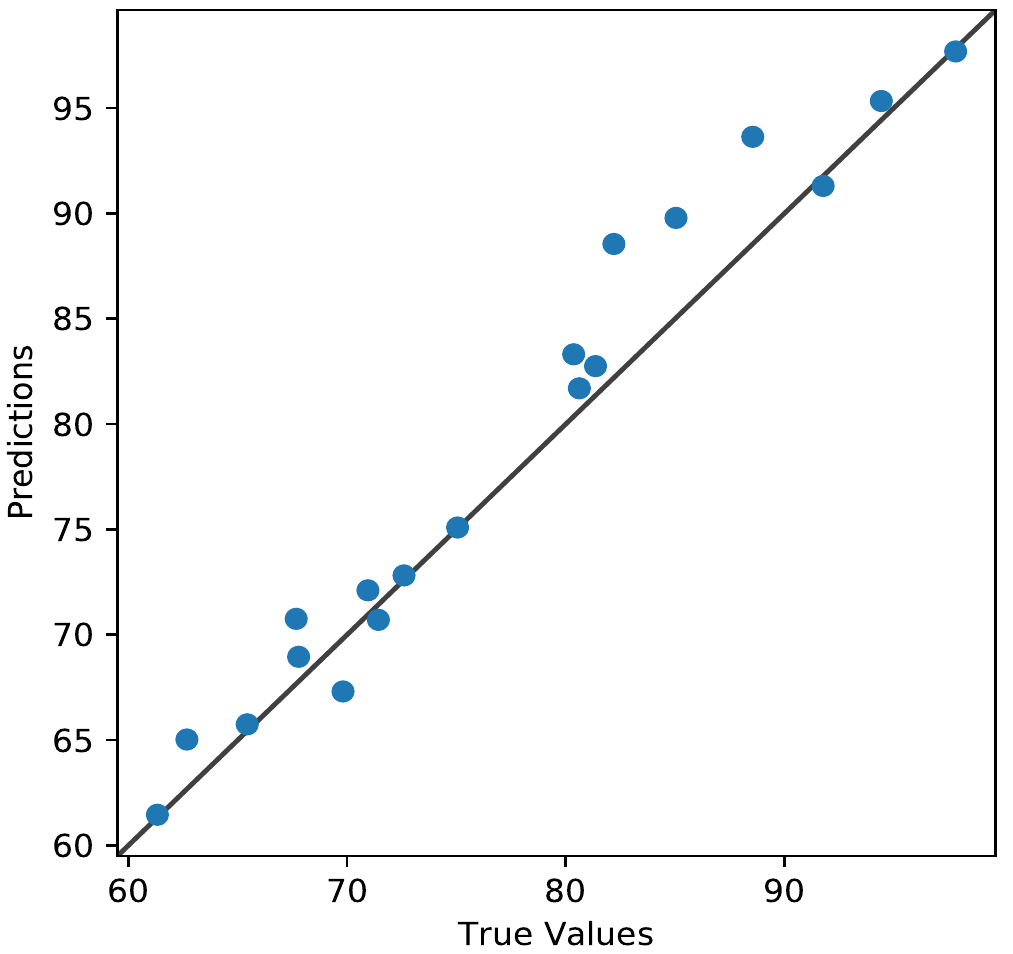
\includegraphics[width=\textwidth]{visualisation/eval_100m.png}
\end{minipage}
\begin{minipage}{0.23\textwidth}
    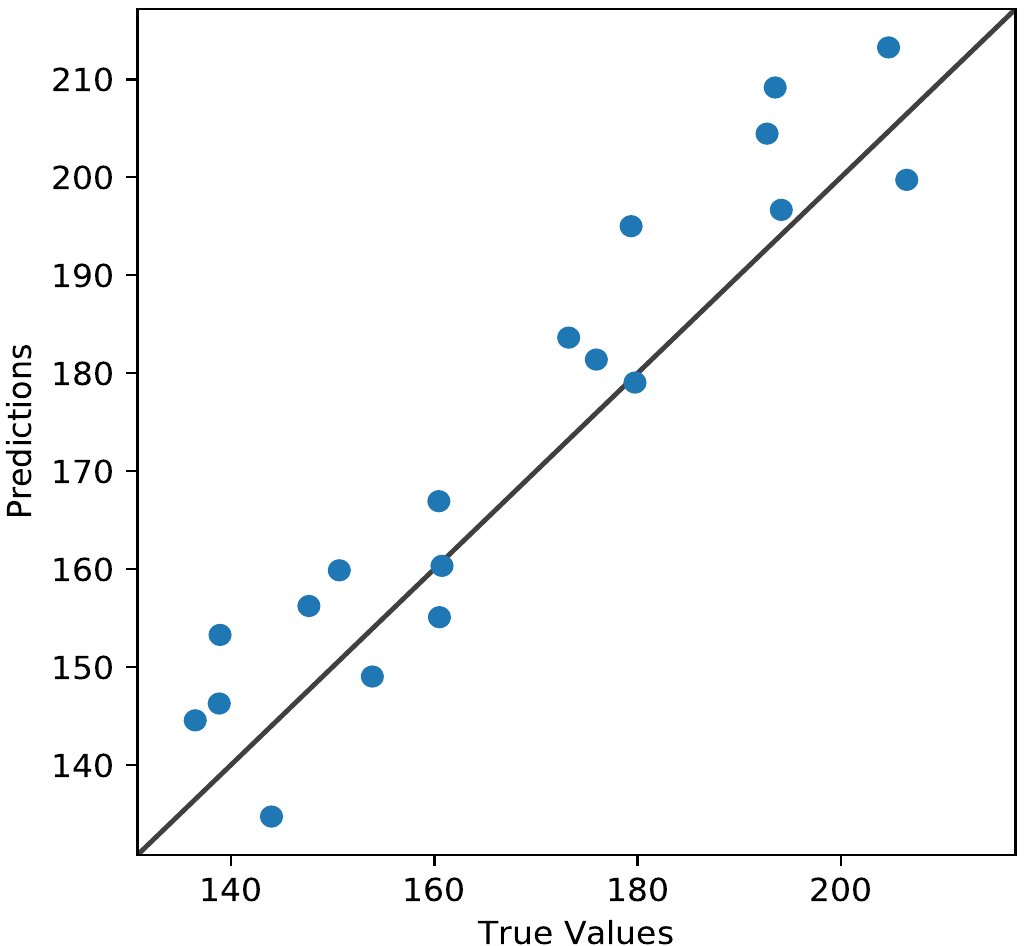
\includegraphics[width=\textwidth]{visualisation/eval_200m.png}
\end{minipage}
\caption{Evaluation of 100m (left) and 200m (right) model}
\label{fig:eval_model}
\end{figure}
The models achieve a mean-absolute error of $1.83$ for the 100m model and $7.97$ for the 200m model. We consider the 100m prediction as successful thus we use this model in our application.\\
The 200m prediction, however, has deficits. A potential improvement could be to include the 100m times in the 200m prediction. In order to evaluate this idea, we train two additional models. For the first model, we add the correct 100m times to the training data and for the second model, we use the 100m model to predict the 100m times and add these times to the training data. Figure \ref{fig:200m_variations} evaluates the four resulting models. The small yellow circles use the correct 100m times for training and prediction. It is important to mention that this model is only for theoretical analysis and does not apply to our real-world problem as we do not know the correct 100m times when we predict new samples. However, this model shows that using the 100m times for the 200m prediction can indeed improve the results. The models using the predicted 100m times for the 200m prediction do not perform better than the original model. Moreover, we can see in the plot that these models almost ignore the 100m time as their predicted times are nearly identical. A reason for this is that the 100m prediction model is not good enough to be helpful for the 200m prediction. Finally, using the 100m times for the 200m model is a good idea but does not work in practice; thus, we use the original 200m model in our application.
\section{Android application}\label{sec:app_plans}
We implement the Android application "SwimPredictor" using Java, a minimum SDK version of 22 and a target SDK version of 28. The app implements three functionalities: The usage of the trained models, a stopwatch to measure the times and a database to store the predicted results and swimmer information to access it later when he makes the competition registration. All three functionalities are implemented as fragments and can be accessed from a bottom tab navigation whats makes changing from one functionality to another very easy and intuitive. Figure \ref{fig:app_screenshots} shows screenshots of the final Android application.\\
\begin{figure}[ht]
\centering
\begin{minipage}{0.2\textwidth}
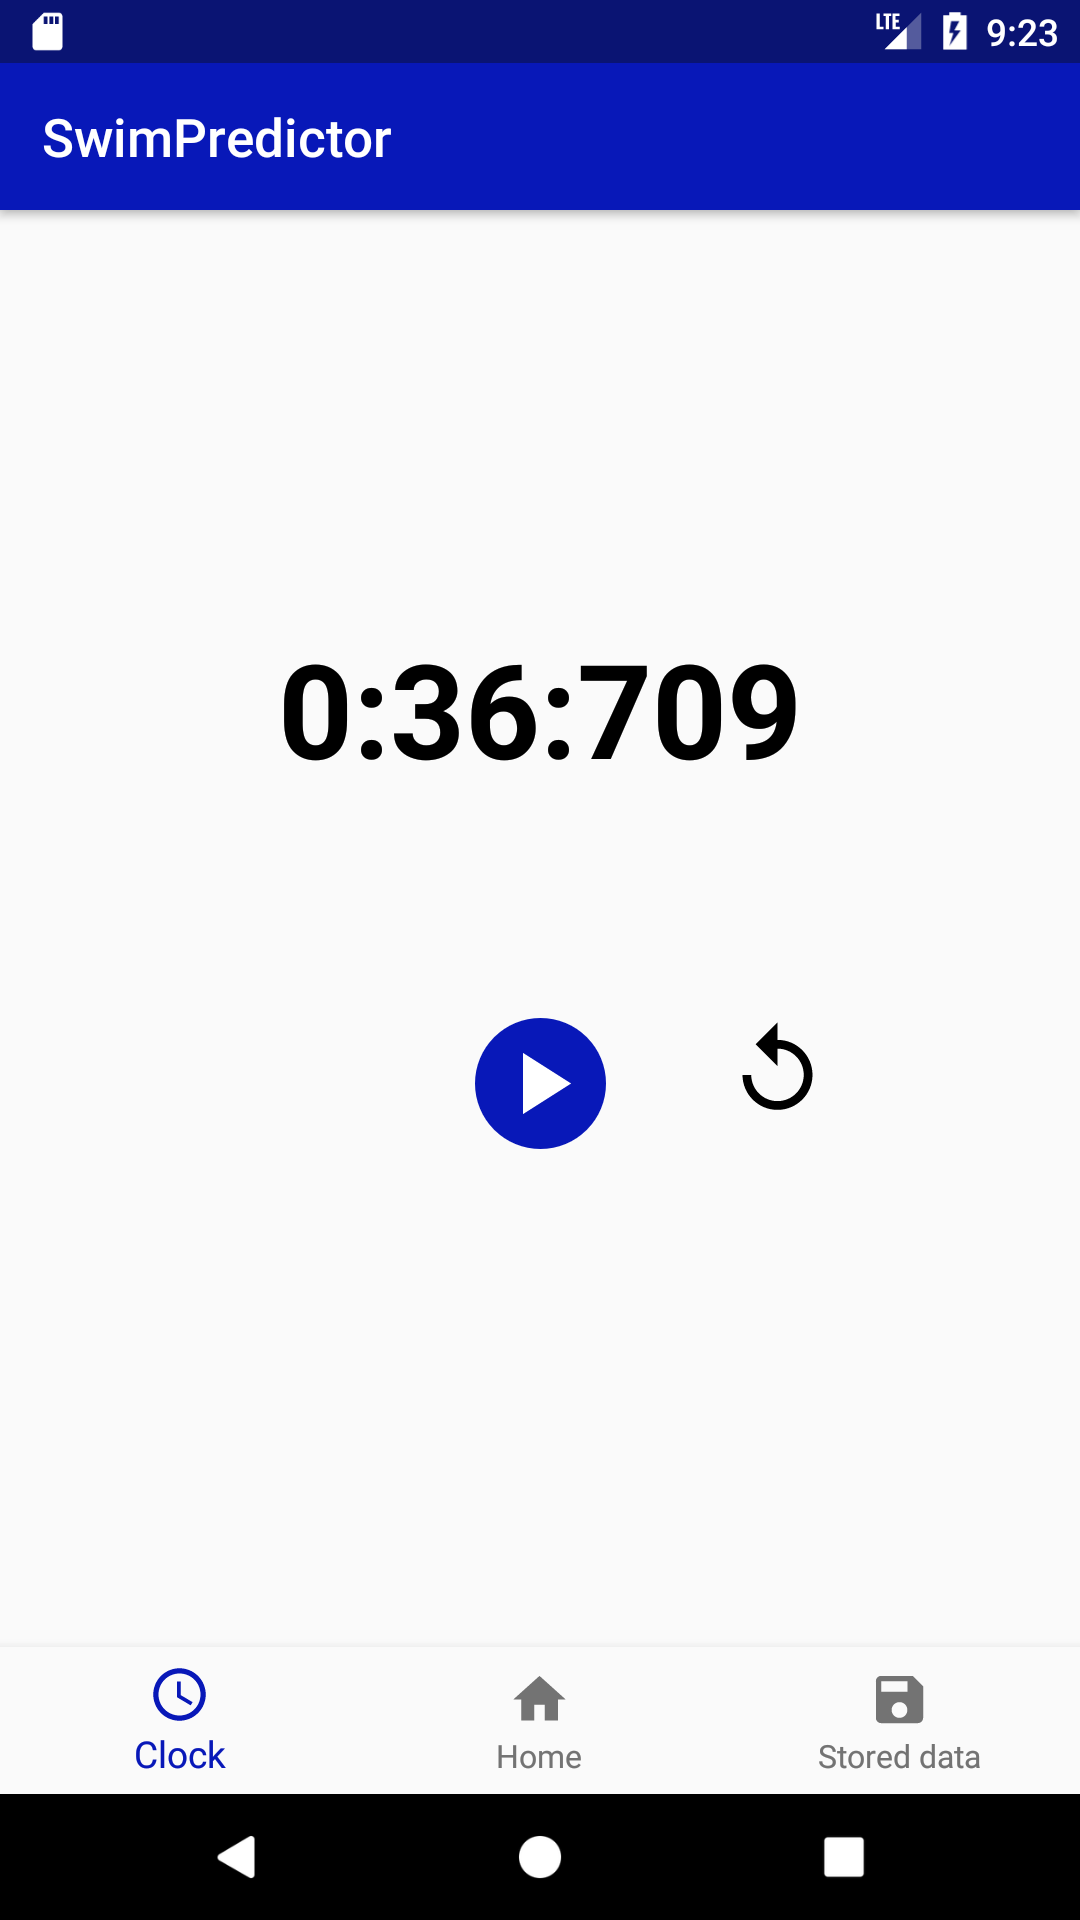
\includegraphics[width=\textwidth]{visualisation/stopwatch_view.png}
\end{minipage}
\begin{minipage}{0.2\textwidth}
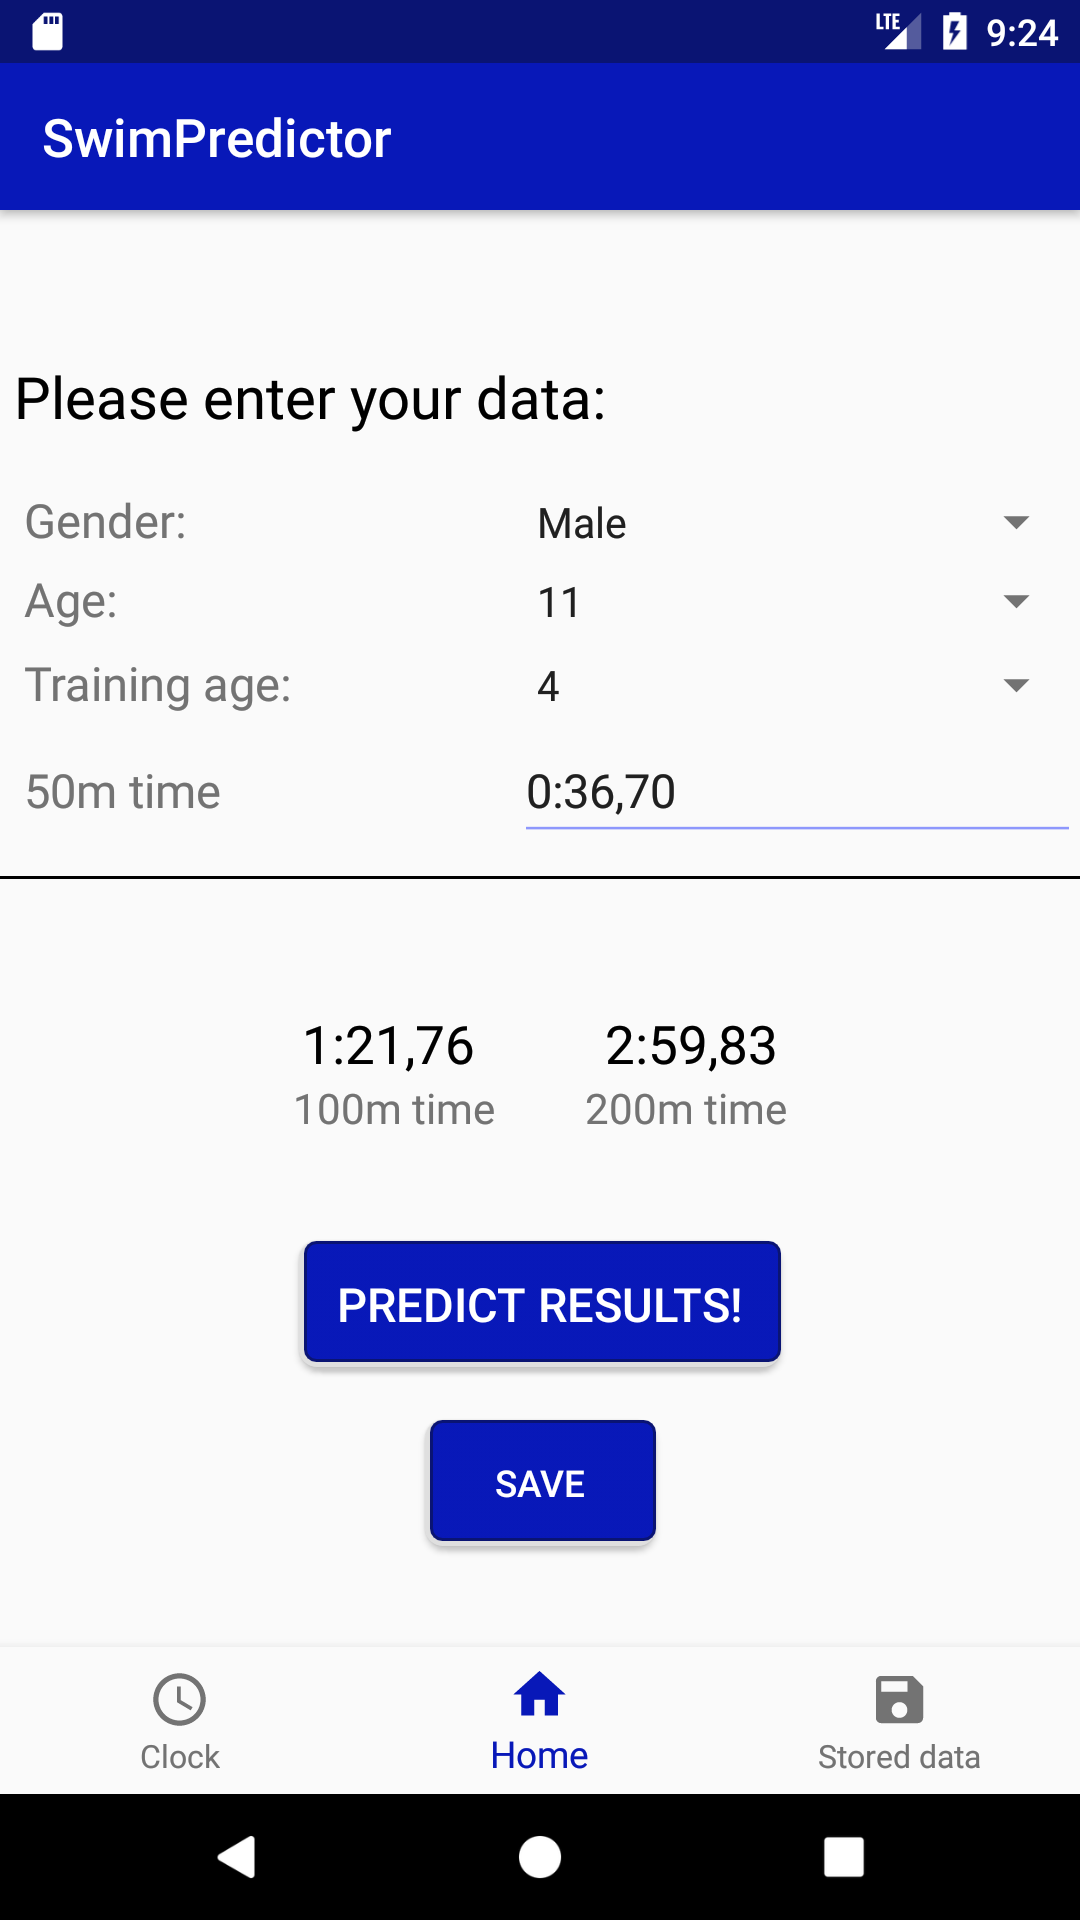
\includegraphics[width=\textwidth]{visualisation/prediction_view.png}
\end{minipage}
\caption{Screenshots of the app's stopwatch and home view}
\label{fig:app_screenshots}
\end{figure}
In the core or home fragment the coach can enter the information of the swimmer and the 50m time he measured in training and let the app predict the longer distance times based on this information. It loads the pre-trained tensorflow-lite model it needs for the predictions from the app's assets folder. To use these models, we need to include the tensorflow-lite library in our app's \texttt{build.gradle} file. The coach can enter the information about the swimmer by choosing values from a dropdown list. This prevents the coach from entering unknown values or values in the wrong format. Moreover, the core fragment has a predict button, with which the user can trigger the prediction, two text views to display the predicted times and a store button to store the current record.\\
The stopwatch function implemented in the \texttt{org.swimpredictor.ui.clock} package has two buttons, a play/pause button and a reset button, as well as a text to display the measured time. We explain the stopwatch logic in Figure \ref{fig:stopwatch_logic}. At first the stopwatch is set to zero. When the play button is clicked, the time starts to run and the play icon on the play/pause button changes to a pause icon. When clicking the pause button, the stopwatch stops running, displays the current time and the button shows the play icon again. The time is saved into a shared preference object and loaded into the 50m time field of the prediction view thus the user does not need to transfer the time himself. The stopwatch can be reset at any time. If the reset button is clicked, the displayed time and the time stored in the shared preferences are set to zero again. We simulate the running stopwatch using a java $Runnable$ object that displays the difference between the start time and the current system time \footnote{\url{https://www.android-examples.com/android-create-stopwatch-example-\ tutorial-in-android-studio/}, accessed 31.12.2019}.\\
\begin{figure}[ht]
    \centering
    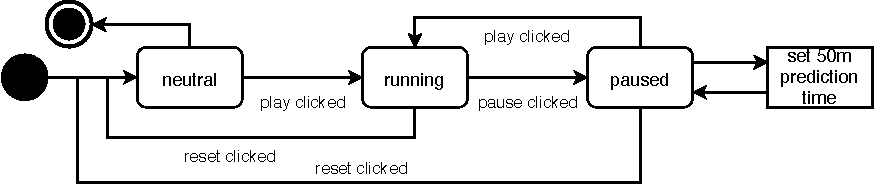
\includegraphics[scale=0.5]{visualisation/StopwatchLogic.pdf}
    \caption{Activity diagram for stopwatch function}
    \label{fig:stopwatch_logic}
\end{figure}
We implement the store functionality in the \texttt{org.swimprodictor.database} package using Android's Room \footnote{\url{https://developer.android.com/training/data-storage/room}, accessed 12.01.2020} and a SQLite database behind it. Although we only have one table, we consider a database the best way to store our data as it is rather easy to implement with Room and it assures consistency by built-in constraints. A \texttt{DataSample} object represents an entity in this table and contains all the information from the data records, as explained in section \ref{sec:data_gen}, together with a unique description that the coach enters when saving a record and human-readable String representation of the times. These Strings have the format \texttt{m:ss,dscs}, e.g. \texttt{1:23,45}. The database itself offers the functionality to insert and delete a sample. The database tab displays all samples stored in the database. We had problems to display the entries in the database as the number of entries in the database changes thus a static TableView is not applicable. Therefore, we use the Open-Source version of the SortableTableView\footnote{\url{https://github.com/ISchwarz23/SortableTableView}, accessed 12.01.2020}. Due to the small display on a mobile device, we were not able to show all information of all samples at the same time. Therefore, the table only shows the description and the three times. The remaining information about the swimmer can be shown in a pop- up message when clicking at the respective sample. To delete a sample, the user needs to long click on the sample he wants to delete. The app then requires a confirmation of the user. If he confirms the deletion, the sample is removed from the database, and the table is reloaded. Figure \ref{fig:app_screenshots_database} shows the TableView of the database entries as well as the pop-up messages with detailed information and deletion confirmation.
\begin{figure}[ht]
\begin{minipage}{0.15\textwidth}
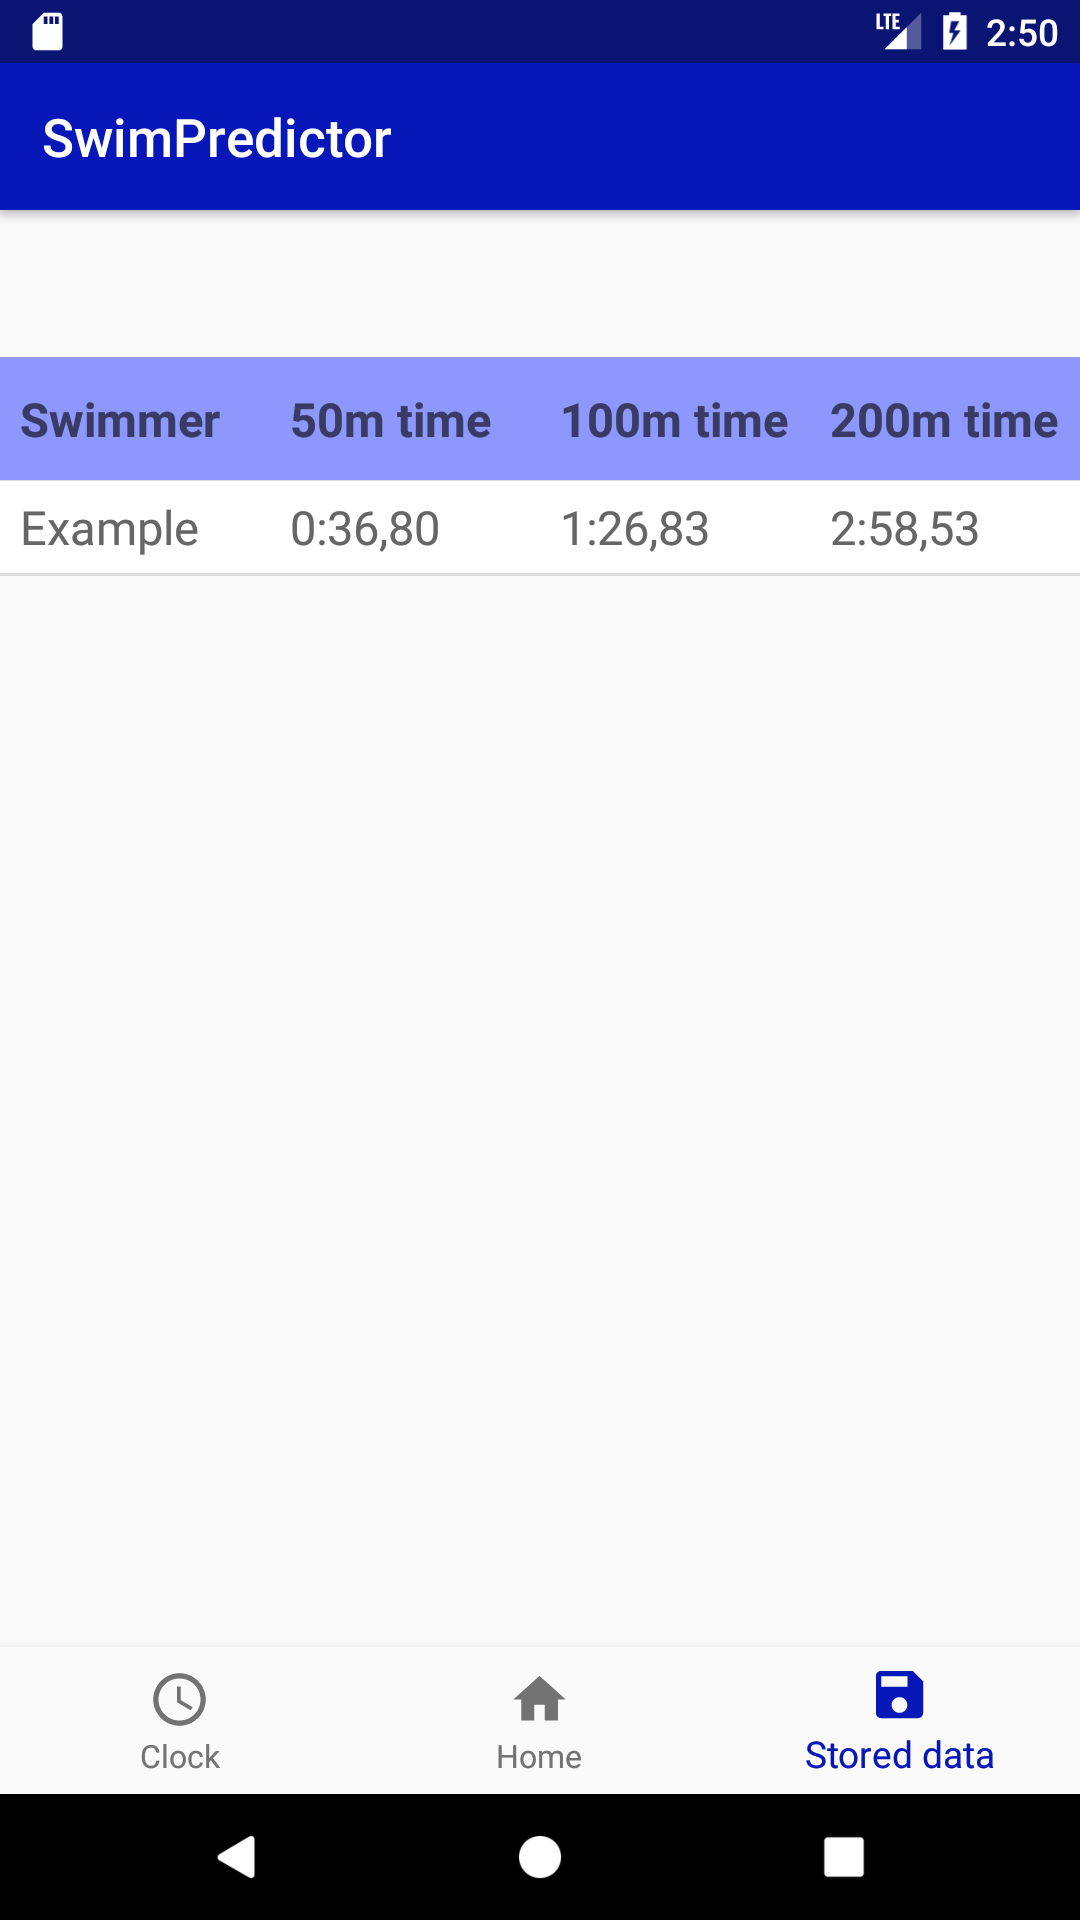
\includegraphics[width=\textwidth]{visualisation/database_view.png}
\end{minipage}
\begin{minipage}{0.15\textwidth}
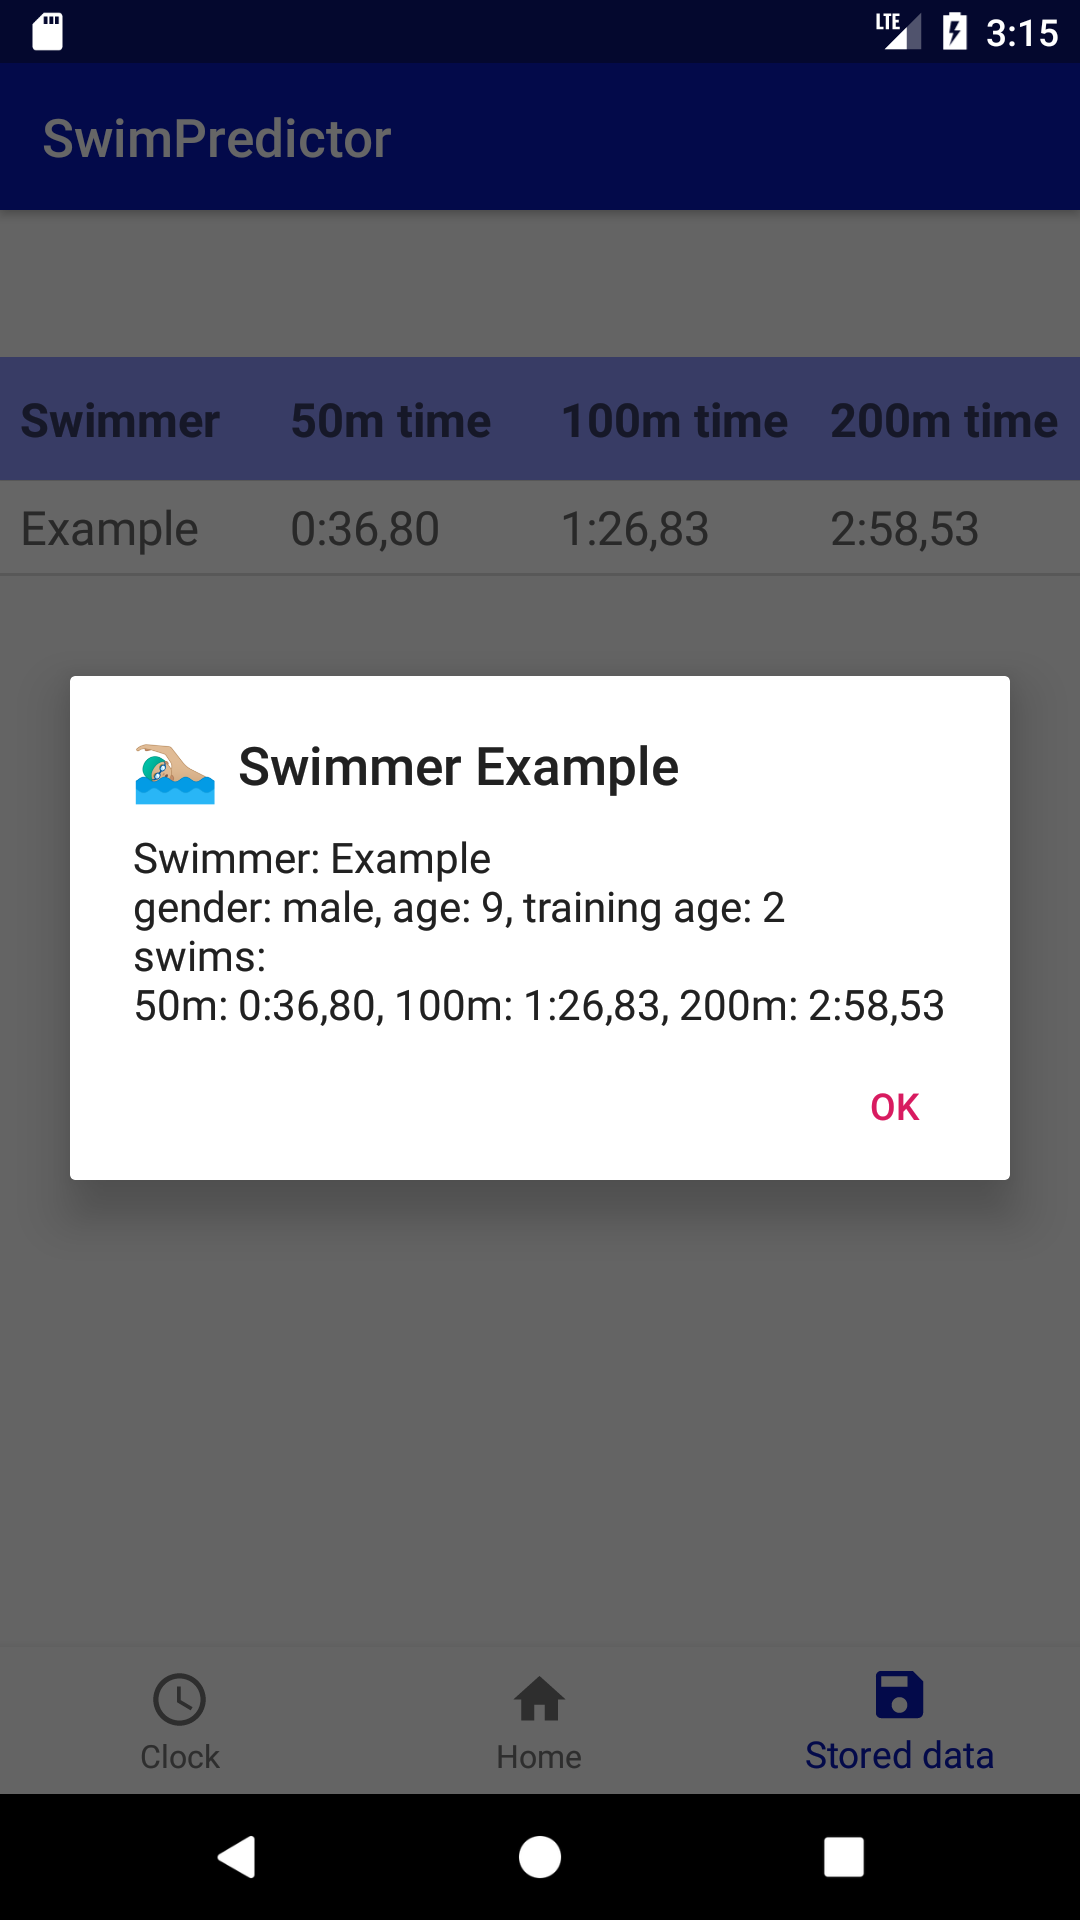
\includegraphics[width=\textwidth]{visualisation/app_detailed_information.png}
\end{minipage}
\begin{minipage}{0.15\textwidth}
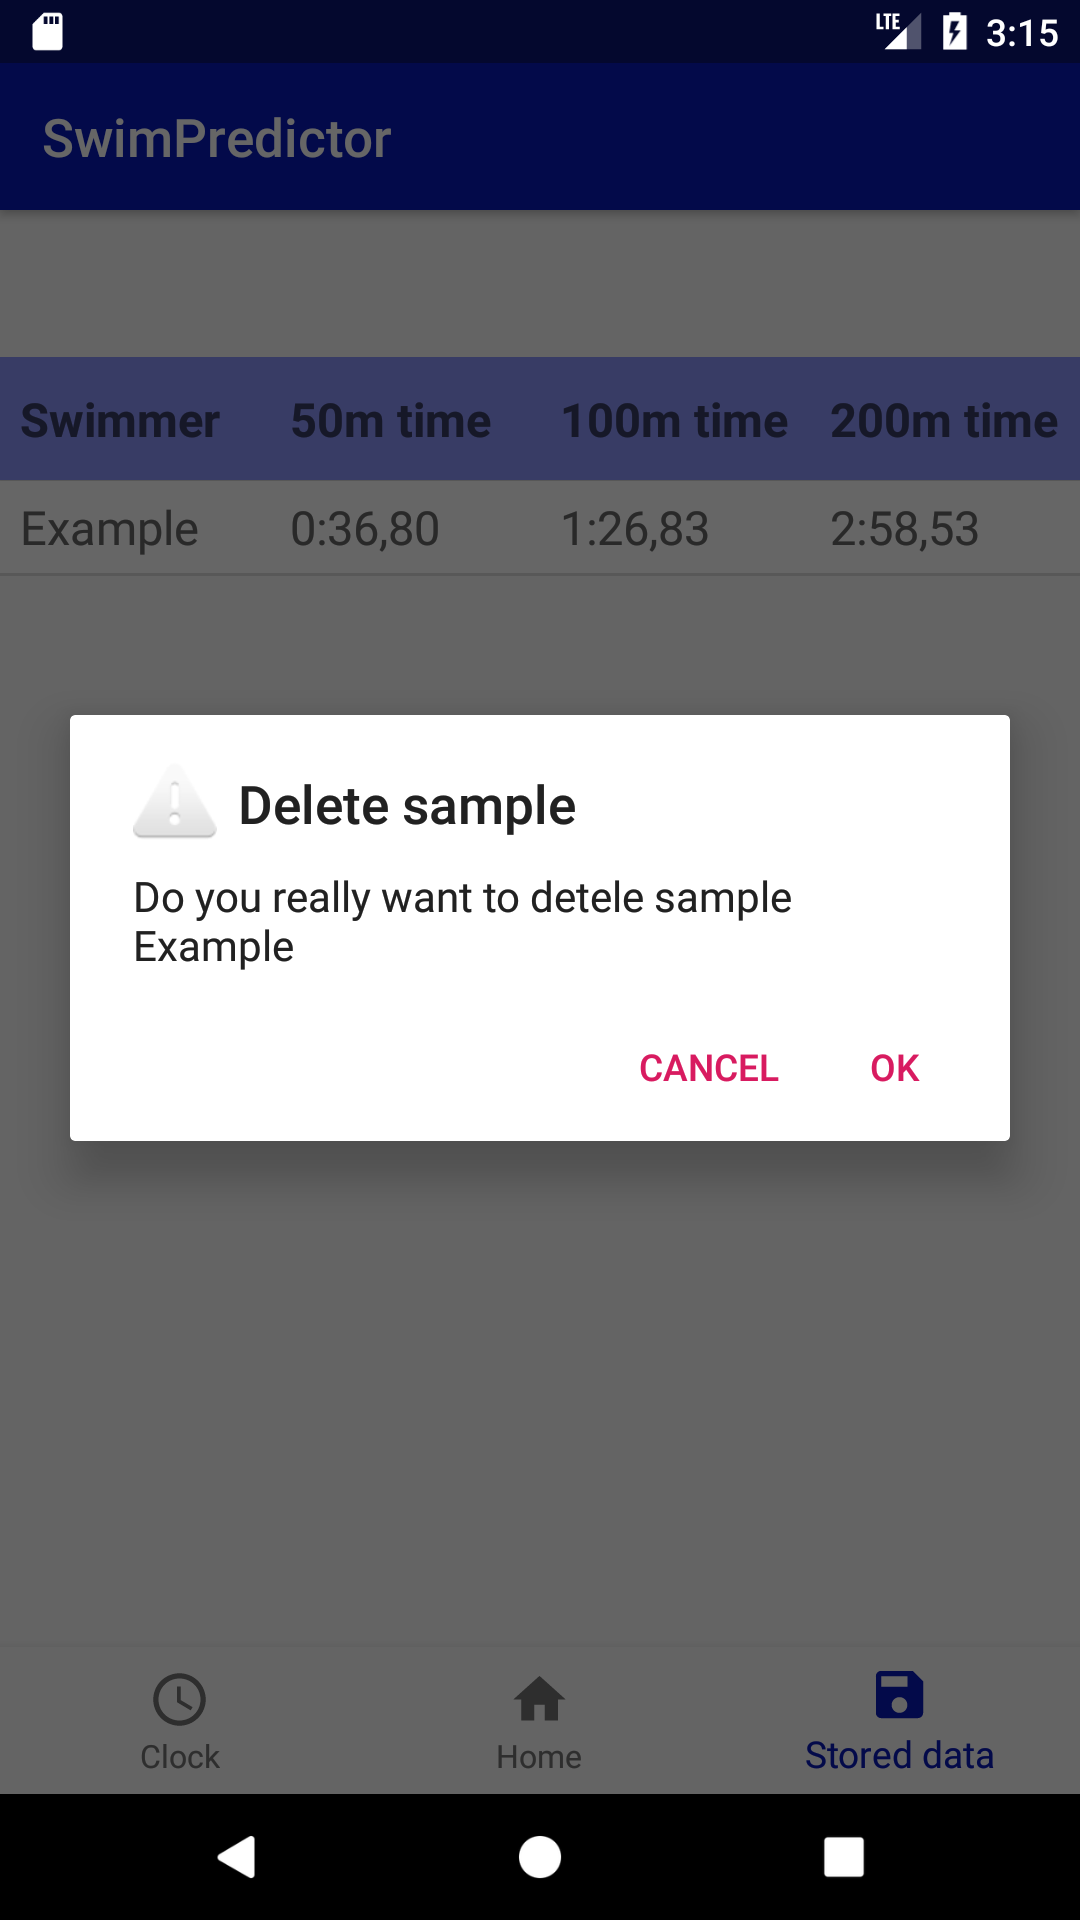
\includegraphics[width=\textwidth]{visualisation/app_confirm_deletion.png}
\end{minipage}
\caption{Screenshots of the app's database functionality}
\label{fig:app_screenshots_database}
\end{figure}
\section{Future Work \& Conclusion}

%\begin{itemize}
%	\item Summarize your thoughts and state your final conclusion about the work you have performed.
%	\item Describe possible future work in the field that is related to you work.
%	\item Detail improvements that could be done to your work in a following project.
%	\item Identify the importance of your work and create an arch to the related work and problem defined in the previous chapters.
%\end{itemize}
In this paper, we introduced an appealing application that helps coaches to estimate their swimmers' performances. However, the underlying machine learning model does not achieve the results we hoped. One reason for this is that we focus on non-professional swimmers; thus, their performance is less constant and therefore, less predictable. Nevertheless, the coaches of these swimmers need the most assistance; thus, a reliable prediction model is of high interest. A possible improvement could be to include more data, especially for the slower 50m times to find a correlation in our data, or use data augmentation to generate more samples from the existing data.\\
Another problem is that the swimmer's performance changes within a season. In our approach, we use an age representation based on the age group of the swimmer instead of his actual age. Therefore, it would be better to include the swimmer's age in month and, more importantly, the information at which point in the season the competition took place.\\
As the related work suggests, the swimmer's anthropometry is of high importance for his performance. Therefore, it would be good to include the height or flexibility in our records. We are currently working on a different approach that includes information about the training status of the swimmer. Therefore, we collect data about the four weeks before the respective competition. This data includes the total amount of training in kilometres as well as the intensity of the training sessions, i.e. the amount of training in the aerobic area or the number of technique sessions. The first results are already promising. However, for this approach, it is indispensable to work together with a group of swimmers as the needed data is not publicly available. \\
To get a first evaluation of our approach, we had to make some constraints. If we find a good data representation to predict results, we can enlarge our predictions to different strokes and distances, as well as include times swam in a 50m pool.
\FloatBarrier
\bibliographystyle{IEEEtranN}
\bibliography{references}

\end{document}
